\chapter{Especificaciones}\label{cap:disenio}

\section{Alcance del Producto}
Este producto está orientado a profesores y tomadores de casos del Patrocinio Jurídico Gratuito, con el fin de facilitar y mejorar la eficiencia del sistema de solicitud y control histórico de los casos, asegurando una experiencia intuitiva en su utilización.

El alcance de esta plataforma abarca el proceso desde la recepción de datos a través de Google Forms, la integración de la información en el sistema, la gestión de los casos en la asignación a comisiones y, finalmente, el seguimiento y gestión de los casos por parte de los profesores de la comisión. 

\subsection{Funciones del Producto}
El sistema desarrollado proporciona un conjunto integral de funciones diseñadas para satisfacer las necesidades específicas de la gestión de casos judiciales y su asignación a las comisiones. Integra de manera fluida con Google Forms, permitiendo la captura eficiente de datos relacionados con casos judiciales y nuevos consultantes. Facilita la selección y asignación de casos a comisiones. La interfaz de usuario intuitiva permite el seguimiento detallado de cada caso a lo largo de su ciclo de vida, facilitando una gestión efectiva y transparente por parte de los profesores de las comisiones. Incluye un sistema de notificaciones vía email y alertas para anunciar ciertos eventos. La interfaz de usuario, es intuitiva, fácil de navegar y brinda una experiencia eficiente, contribuyendo a mejorar la eficiencia, la transparencia y la efectividad en la gestión de casos y la selección de comisiones.

\subsection{Tipos de Usuarios y Características}
El sistema contempla varios tipos de usuarios, cada uno con funciones y características específicas para satisfacer sus necesidades dentro del proceso. Los roles principales incluyen:

\textbf{Administradores del Sistema}: Tienen acceso completo al sistema y la capacidad de gestionar usuarios y acceder a todas las funcionalidades. Su función principal es garantizar el correcto funcionamiento y la configuración adecuada del sistema.

\textbf{Profesores de Comisión}: Estos usuarios son responsables de revisar, evaluar y gestionar los casos asignados a su comisión. Pueden acceder a la información detallada de cada caso, realizar comentarios, asignar tareas y seguir el progreso de manera integral.

\textbf{Solicitantes}: Son los usuarios encargados de presentar casos judiciales mediante Google Forms. Aunque no tienen acceso directo a la plataforma, desempeñan un papel crucial al ingresar casos y nuevos consultantes a través de Google Forms, contribuyendo así al flujo eficiente de datos en el sistema.

\textbf{Administradores de Casos}: Más conocidos como \textbf{Tomadores de Caso}, este rol se ocupa de la gestión específica de los casos, desde su recepción hasta su asignación a una comisión. Pueden revisar la información proporcionada por los solicitantes y asignar casos a las comisiones correspondientes.




\subsection{Entorno Operativo}

La plataforma estará diseñada para operar en un entorno que cumpla con los siguientes requisitos:

\subsubsection{Requisitos de Servidor}
La aplicación está diseñada para ser accesible desde cualquier dispositivo con capacidad para ejecutar contenedores Docker, lo que incluye sistemas operativos como Linux, Windows y macOS. Además, gracias a la naturaleza de Docker, la aplicación es altamente compatible con entornos en la nube, lo que significa que puede ejecutarse en servicios cloud. La orquestación de contenedores también se simplifica mediante tecnologías como Kubernetes; por ejemplo, puede implementarse y gestionarse en servicios como Amazon EKS en AWS.

Se recomienda empezar al menos con:
\begin{itemize}
    \item 6 GB de RAM
    \item 2 núcleo de CPU
\end{itemize}
El almacenamiento de la aplicación dependerá de la cantidad de registros almacenados de las consultas, ya que se almacenan directamente en el servidor.

Estos requisitos proporcionarán una base para el despliegue inicial de la aplicación, asegurando un funcionamiento estable y eficaz. Se debe tener en cuenta que estos son requisitos mínimos y se puede considerar la posibilidad de cambiar estos recursos en función de la carga de trabajo y el crecimiento futuro de la aplicación.

\subsubsection{Navegadores Soportados}

\begin{itemize}
    \item Google Chrome. Se probó en la versión Versión 120.0.6099.130.
    \item Mozilla Firefox. Se probó en la versión 121.0.
\end{itemize}

\subsubsection{Conectividad}
Se requiere una conexión a Internet estable para el correcto funcionamiento de la integración con Google Forms y el acceso a la plataforma. La velocidad de la conexión afectará directamente la eficiencia en la carga y manejo de datos.

\subsubsection{Dispositivos Compatibles}
La plataforma está diseñada para ser accesible desde dispositivos con pantallas de tamaño mediano a grande, como computadoras de escritorio, laptops y tabletas. El acceso desde dispositivos móviles puede ser posible, pero la experiencia de usuario puede variar según el tamaño de la pantalla.


\section{Requerimientos Funcionales}
En el marco de este proyecto, los requerimientos funcionales se agrupan según sus funcionalidades específicas:

\begin{table}[H]
\centering
\begin{tabular}{|l|l|}
\hline
\textbf{Referencia} & \textbf{Función} \\
\hline
\textbf{RF.1} & Sistema de solicitudes de asignación de casos \\
\hline
\textbf{RF.2} & Sistema de gestión de casos por comisión \\
\hline
\textbf{RF.3} & Sistema de registro de consultantes y consultas \\
\hline
\textbf{RF.4} & Sistema de alertas y notificaciones \\
\hline
\textbf{RF.5} & Registro y Autenticación de Usuarios \\
\hline
\end{tabular}
\caption{Requerimientos Funcionales}
\label{tab:rf}
\end{table}


\section{Diagrama de Caso de Uso del Sistema}
A continuación, se presentan los diagramas de caso de uso \ref{fig:caso-de-uso} para identificar a los actores implicados en una interacción. Si bien en este caso no se relacionan los casos de uso a alto nivel con diferentes actores, no significa que no exista una relación. Por otro lado, debe entenderse que Google Forms también cumple un rol e interactúa con el sistema principal Case Management System.

\begin{figure}[H]
\centering
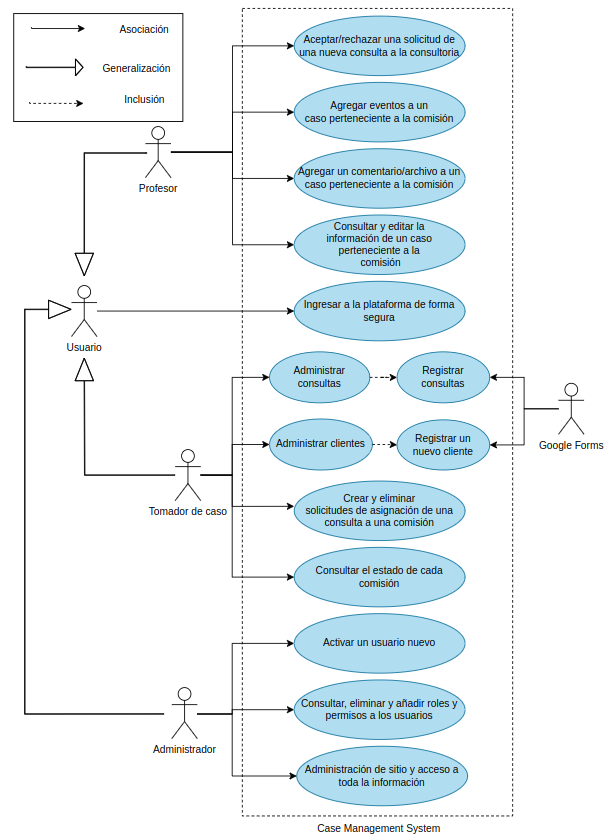
\includegraphics[width=1\linewidth]{fig/caso-de-uso.png}
\caption{Diagrama Caso de Uso}
\label{fig:caso-de-uso}
\end{figure}

\begin{itemize}
\item \textbf{CU.1}: Aceptar/rechazar una solicitud de una nueva consulta a la consultoría.
\item \textbf{CU.2}: Agregar eventos a un caso perteneciente a la comisión.
\item \textbf{CU.3}: Agregar un comentario/archivo a un caso perteneciente a la comisión.
\item \textbf{CU.4}: Ingresar a la plataforma de forma segura.
\item \textbf{CU.5}: Administrar consultas.
\item \textbf{CU.6}: Administrar consultantes.
\item \textbf{CU.7}: Crear y eliminar solicitudes de asignación de una consulta a una comisión.
\item \textbf{CU.8}: Ver el estado de cada comisión.
\item \textbf{CU.9}: Activar a un usuario nuevo.
\item \textbf{CU.10}: Administrar roles y permisos de los usuarios.
\item \textbf{CU.11}: Administración de sitio y acceso a toda la información.
\end{itemize}


\section{Diagrama de Secuencia Nominal Simplificado}
A continuación, se incluyen los diagramas de secuencia \ref{fig:secuencia-registro} y \ref{fig:secuencia-nominal} de alto nivel para agregar comprensión a la funcionalidad de cada actor y su interacción con otros actores.

\begin{figure}[H]
\centering
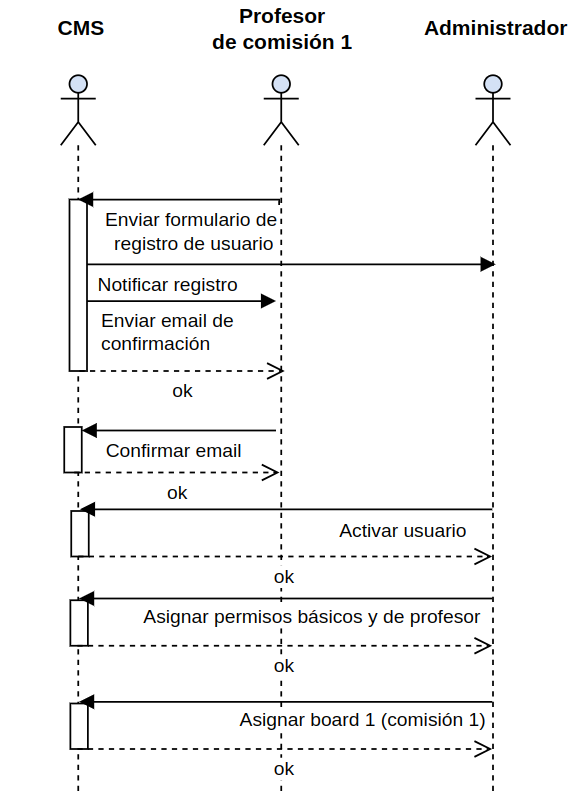
\includegraphics[width=0.5\linewidth]{fig/secuencia-registro.png}
\caption{Diagrama de Secuencia Para Registro de Usuario}
\label{fig:secuencia-registro}
\end{figure}
En este diagrama, participa el sistema Case Management System, el profesor de la comisión número uno y el jefe de patrocinio o administrador.

\begin{figure}[H]
\centering
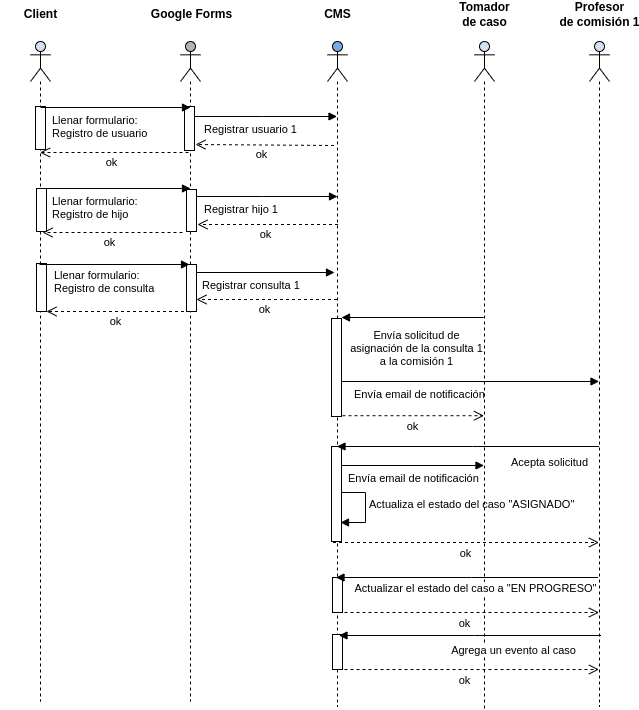
\includegraphics[width=1\linewidth]{fig/secuencia-basica.png}
\caption{Diagrama de Secuencia Simplificado}
\label{fig:secuencia-nominal}
\end{figure}
En este diagrama, participan varios actores, incluyendo un consultante con un solo hijo, el sistema externo Google Forms, el sistema Case Management System, el usuario tomador de caso, el profesor de la comisión número uno y el jefe de patrocinio o administrador.

